\documentclass[
	% -- opções da classe memoir --
	12pt,				% tamanho da fonte
	openright,			% capítulos começam em pág ímpar (insere página vazia caso preciso)
	oneside,			% para impressão em frente e verso. Oposto a oneside
	a4paper,			% tamanho do papel.
	% -- opções da classe abntex2 --
	chapter=TITLE,		% títulos de capítulos convertidos em letras maiúsculas
	%section=TITLE,		% títulos de seções convertidos em letras maiúsculas
	%subsection=TITLE,	% títulos de subseções convertidos em letras maiúsculas
	%subsubsection=TITLE,% títulos de subsubseções convertidos em letras maiúsculas
	% -- opções do pacote babel --
	english,			% idioma adicional para hifenização
	french,				% idioma adicional para hifenização
	spanish,			% idioma adicional para hifenização
	brazil				% o último idioma é o principal do documento
	]{abntex2}
% ---
% Pacotes básicos 
% ---
\usepackage{lmodern}			% Usa a fonte Latin Modern
\usepackage{mathptmx}			% Usa a fonte Times New Roman
\usepackage[T1]{fontenc}		% Selecao de codigos de fonte.
\usepackage[utf8]{inputenc}		% Codificacao do documento (conversão automática dos acentos)
\usepackage{lastpage}			% Usado pela Ficha catalográfica
\usepackage{indentfirst}		% Indenta o primeiro parágrafo de cada seção.
\usepackage{color}				% Controle das cores
\usepackage{graphicx}			% Inclusão de gráficos
\usepackage{subcaption}				% Inclusão de gráficos lado a lado
\usepackage{microtype} 			% para melhorias de justificação
\usepackage{tabularx,ragged2e}	% Para inserir tabelas
\usepackage{multirow}			% Para mesclar células
\usepackage[dvipsnames,table,xcdraw]{xcolor}		% Permite adicionar cores nas linhas de tabelas
\usepackage{fancyvrb}			% Permite adicionar arquivos de texto
\usepackage[portuguese, ruled, linesnumbered]{algorithm2e} % Uso de algoritmos
\usepackage{amsfonts}			% Permite usar notação de conjuntos
\usepackage{amsmath}			% Permite citar equações
\usepackage{amsthm}				% Permite criar teoremas e experimentos
\usepackage[font={bf, small}, labelsep=endash, labelfont=bf]{caption}	% Faz legenda de figuras ficarem em negrito
\usepackage{cancel}				% Permite fazer expressão tendendo a zero
\usepackage{epstopdf}			% Converte eps para pdf
\usepackage[final]{pdfpages}
\usepackage{float}


\usepackage{listings}
\usepackage{xcolor}
\usepackage{lipsum}

\newcolumntype{L}{>{\RaggedRight\arraybackslash}X}
% ---
% ---
% Pacotes adicionais, usados apenas no âmbito do Modelo Canônico do abnteX2
% ---
\usepackage{lipsum}				% para geração de dummy text
% ---
% ---
% Pacotes de citações
% ---
%\usepackage[brazilian,hyperpageref]{backref}	 % Paginas com as citações na bibl
\usepackage[alf, abnt-emphasize=bf]{abntex2cite}	% Citações padrão ABNT
% ---
% Customizações para o layout da UFPA
% ---
\usepackage{modelo-ufpa/ufpa}
% Muda o título de lista de ilustrações para lista de figuras
\addto\captionsbrazil{%
  \renewcommand{\listfigurename}%
    {Lista de Ilustrações}%
	\renewcommand{\listtablename}%
    {Lista de Tabelas}%
}
% Permite utilizar figuras sem precisar colocar o caminho absoluto
\graphicspath{{imagens/}}
% Define o ambiente de experimentos
\theoremstyle{definition}
\newtheorem{experimento}{Experimento}[section]
\newcommand{\experimentoautorefname}{Experimento}


% --------------------------------------------------------------
% Informações do TRABALHO
% --------------------------------------------------------------
\universidade{UNIVERSIDADE FEDERAL DO PARÁ}
\instituto{INSTITUTO DE TECNOLOGIA}
\faculdade{FACULDADE DE COMPUTAÇÃO E TELECOMUNICAÇÕES}
%\curso{CURSO DE BACHARELADO EM SISTEMAS DE INFORMAÇÃO}
\titulo{RELATÓRIO DE SISTEMAS OPERACIONAIS}
\autor{
%\begin{tabular}{l l}
    DAVID PINHEIRO DE SOUSA - 202207040045 \\
    JOAO VICTOR SANTOS BRITO FERREIRA - 202207040028 \\
    JOEL TAVARES MIRANDA - 202206840054 \\
    KAUAN MIRANDA TAVARES - 202206840033 \\
    MARCO ANTONIO DO ESPIRITO SANTO MAUES JUNIOR - 202206840038 \\
%\end{tabular}
}
\local{Belém}
\data{2023}
\orientador{Prof. Dr. Diego Lisboa Cardoso}
\tipotrabalho{Monografia}

% o nome da instituição e a área de concentração 
\preambulo{Relatório do trabalho 5 de Sistemas Operacionais.}
%\sobrenome{Sobrenome}
%\nome{Nome}
%\palavraschave
%\datadadefesa{Data da Defesa: 09 de Março de 2017}%07 de Dezembro de 2016}
\conceito{Conceito: Excelente}
\faculdadedoorientador{Faculdade de Biotecnologia - UFPA}
\primeiromembrodabanca{Prof. Dr. Nome Sobrenome}
\faculdadedoprimeiromembrodabanca{Faculdade de Computação - UFPA}
\segundomembrodabanca{Prof. Dra. Nome Sobrenome}
\faculdadedosegundomembrodabanca{Faculdade de Biotecnologia - UFPA}
% -------------------------------------------------------------------------
% ---
% Configurações de aparência do PDF final
% alterando o aspecto da cor azul
\definecolor{blue}{RGB}{41,5,195}
% informações do PDF
\makeatletter
\hypersetup{
     	%pagebackref=true,
		pdftitle={\imprimirtitulo}, 
		pdfauthor={\imprimirautor},
    	pdfsubject={\imprimirpreambulo},
	    pdfcreator={LaTeX with abnTeX2},
		pdfkeywords={\imprimirpalavraschave}, 
		colorlinks=true,       		% false: boxed links; true: colored links
    	linkcolor=black,          	% color of internal links
    	citecolor=black,        		% color of links to bibliography
    	filecolor=magenta,      		% color of file links
		urlcolor=blue,
		bookmarksdepth=4,
        breaklinks=true
}
\makeatother
% --- 
% Espaçamentos entre linhas e parágrafos 
% --- 
% O tamanho do parágrafo é dado por:
\setlength{\parindent}{1.3cm}
% Controle do espaçamento entre um parágrafo e outro:
\setlength{\parskip}{0.2cm}  % tente também \onelineskip
% compila o indice
% ---
\makeindex
% ---

% -------------------------------------------------------------------------
% ---------------------------INICIO DO DOCUMENTO---------------------------
% -------------------------------------------------------------------------
\begin{document}
% Seleciona o idioma do documento (conforme pacotes do babel)
\selectlanguage{brazil}
% Retira espaço extra obsoleto entre as frases.
\frenchspacing 
% ----------------------------------------------------------
% ELEMENTOS PRÉ-TEXTUAIS
% ----------------------------------------------------------
% \pretextual

% ---
% Capa
% ---
\imprimircapa
% ---

% ---
% Folha de rosto
% ---
\imprimirfolhaderosto
% ---

% ---
% Inserir a ficha bibliografica
% ---

\newpage



% ---
% Inserir errata
% ---

% ---

% ---
% Inserir folha de aprovação
% ---

% Isto é um exemplo de Folha de aprovação, elemento obrigatório da NBR
% 14724/2011 (seção 4.2.1.3). Você pode utilizar este modelo até a aprovação
% do trabalho. Após isso, substitua todo o conteúdo deste arquivo por uma
% imagem da página assinada pela banca com o comando abaixo:
%
% \includepdf{folhadeaprovacao_final.pdf}
%

% ---

% ---
% Dedicatória
% ---


% ---
% Agradecimentos
% ---
% ---

% ---
% Epígrafe
% ---


% ---
% RESUMOS
% ---

% resumo em português
\setlength{\absparsep}{18pt} % ajusta o espaçamento dos parágrafos do resumo




% ---

% ---

% ---

% ---
% inserir lista de quadros
% ---

% ---


% ---
% inserir lista de abreviaturas e siglas


% ---
% inserir lista de símbolos
% ---


% ---
% inserir o sumario
% ---
\pdfbookmark[0]{\contentsname}{toc}
\tableofcontents*
\cleardoublepage
% ---



% ----------------------------------------------------------
% ELEMENTOS TEXTUAIS
% ----------------------------------------------------------
\textual

% ----------------------------------------------------------
% Introdução
% ----------------------------------------------------------

\chapter{Introdução}

O gerenciamento eficiente da memória é uma parte crucial do desempenho de sistemas operacionais, 
especialmente em ambientes com recursos limitados. A memória swap, ou memória virtual, desempenha um papel fundamental ao 
oferecer recursos adicionais para armazenamento temporário quando a memória RAM atinge seus limites.

Este estudo se concentra em explorar o impacto do uso de swap em aplicações que demandam 
uma quantidade significativa de memória RAM. Em ambientes onde a memória física disponível 
é restrita, a utilização eficaz da memória swap pode influenciar diretamente o desempenho 
e a responsividade do sistema.

\chapter{Objetivos}

O presente estudo tem como objetivos:

\begin{itemize}
    \item Analisar o impacto do uso de memória swap em aplicações que demandam uma quantidade significativa de memória RAM.
    \item Investigar a medida em que a adição de memória swap é ou deixa de ser eficiente para o sistema testando múltiplos cenários de swap.
\end{itemize}


\chapter{Desenvolvimento} \label{chap:des}

Neste capítulo, é descrito o desenvolvimento da aplicação em python feita para medir a eficácia do uso de swap. 
O objetivo principal desta aplicação é simular um cenário de carga de trabalho intensiva em 
RAM, onde a demanda por recursos de memória é significativamente elevada e posteriormente avaliar a 
execução da aplicação nos seguintes 3 cenários distintos de swap:

\begin{enumerate}
    \item \textbf{Sem Swap (0gb):} A execução sem o uso de swap, onde toda a carga é tratada pela RAM principal.
    \item \textbf{Swap Igual à RAM (8gb):} A execução com uma configuração de swap equivalente à capacidade da RAM disponível.
    \item \textbf{Swap duas vezes maior que a RAM (16gb):} A execução com uma configuração de swap que é o dobro da capacidade da RAM disponível.
\end{enumerate}
%Em cada cenário será visto através de gráficos como o uso de swap influencia o desempenho da aplicação 
%em termos de tempo de execução e eficiência no uso de recursos de memória.

\section{Código em Python}

Na figura \ref{fig:swapy} é mostrada a aplicação desenvolvida que consiste na realização de operações 
com matrizes, uma tarefa conhecida por consumir grandes quantidades de memória. O propósito principal 
é replicar um ambiente sob uso voraz.

\begin{figure}[H]
	\centering
	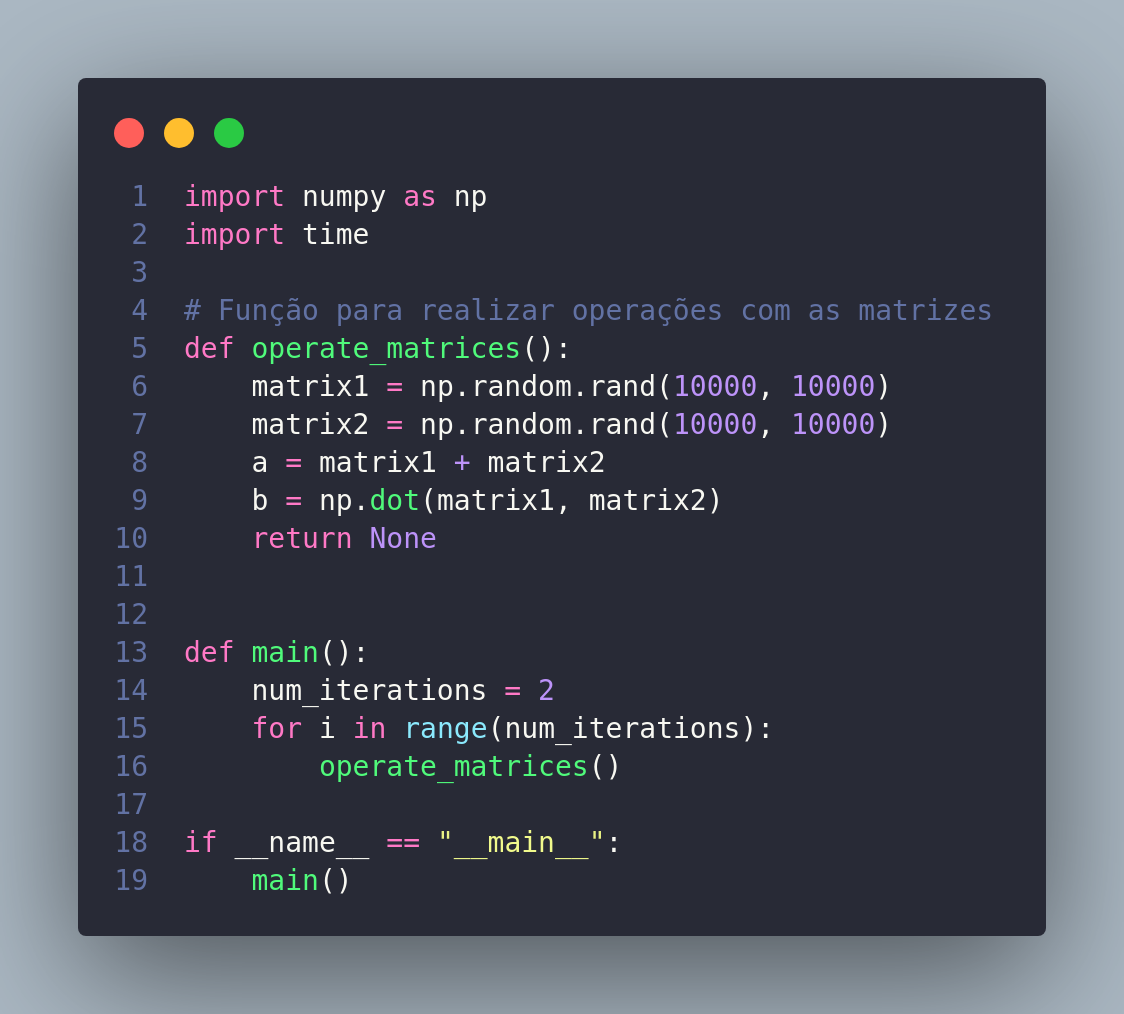
\includegraphics[width=0.6\textwidth]{swapy.png}
	\caption{Código em Python. Disponível em \href{https://github.com/jvictorferreira3301/Sistemas_Operacionais/blob/main/5_swap/memoria_swap.py}{github.com/jvictorferreira3301/SistemasOperacionais
	/blob/main/5\_swap/memoria\_swap.py}}
	\label{fig:swapy}
\end{figure}


O código em questão (\ref{fig:swapy}) realiza operações com matrizes usando a biblioteca NumPy em Python. 
Abaixo, estão os principais pontos do código explicados:

\begin{itemize}[label=--]
    \item \textbf{Importação de Bibliotecas:}
    \begin{itemize}
        \item \texttt{import numpy as np}: Importa a biblioteca NumPy e a renomeia como \texttt{np} para facilitar o uso.
        \item \texttt{import time}: Importa a biblioteca \texttt{time} para medir o tempo de execução (embora essa funcionalidade não seja usada no código atual).
    \end{itemize}
    
    \item \textbf{Definição da Função \texttt{operate\_matrices}:}
    \begin{itemize}
        \item Gera duas matrizes aleatórias de tamanho \(10000 \times 10000\), denominadas \texttt{matrix1} e \texttt{matrix2}.
        \item Realiza duas operações com as matrizes:
        \begin{itemize}
            \item \texttt{a = matrix1 + matrix2}: Soma elemento por elemento das duas matrizes.
            \item \texttt{b = np.dot(matrix1, matrix2)}: Calcula o produto ponto a ponto das duas matrizes.
        \end{itemize}
        \item Retorna \texttt{None}.
    \end{itemize}
    
    \item \textbf{Função \texttt{main}:}
    \begin{itemize}
        \item Define o número de iterações como \texttt{num\_iterations = 2}.
        \item Realiza um loop \texttt{for} com \texttt{num\_iterations} chamando a função \texttt{operate\_matrices} em cada iteração.
    \end{itemize}
    
    \item \textbf{Condição \texttt{if \_\_name\_\_ == "\_\_main\_\_":}}
    \begin{itemize}
        \item Garante que o código dentro deste bloco seja executado apenas se o script for executado como um programa independente, não se for importado como um módulo.
        \item Chama a função \texttt{main()} para iniciar a execução do programa.
    \end{itemize}
\end{itemize}

\section{Obtenção dos Dados para Análise}

Para coletar os dados do uso do swap nos 3 cenários descritos anteriormente (\ref{chap:des}), foi feito um script em bash que é mostrado na figura \ref{fig:swapy}. 
O script em Bash realiza uma série de testes de desempenho relacionados à utilização de memória 
swap em um ambiente Linux.

\begin{figure}[H]
	\centering
	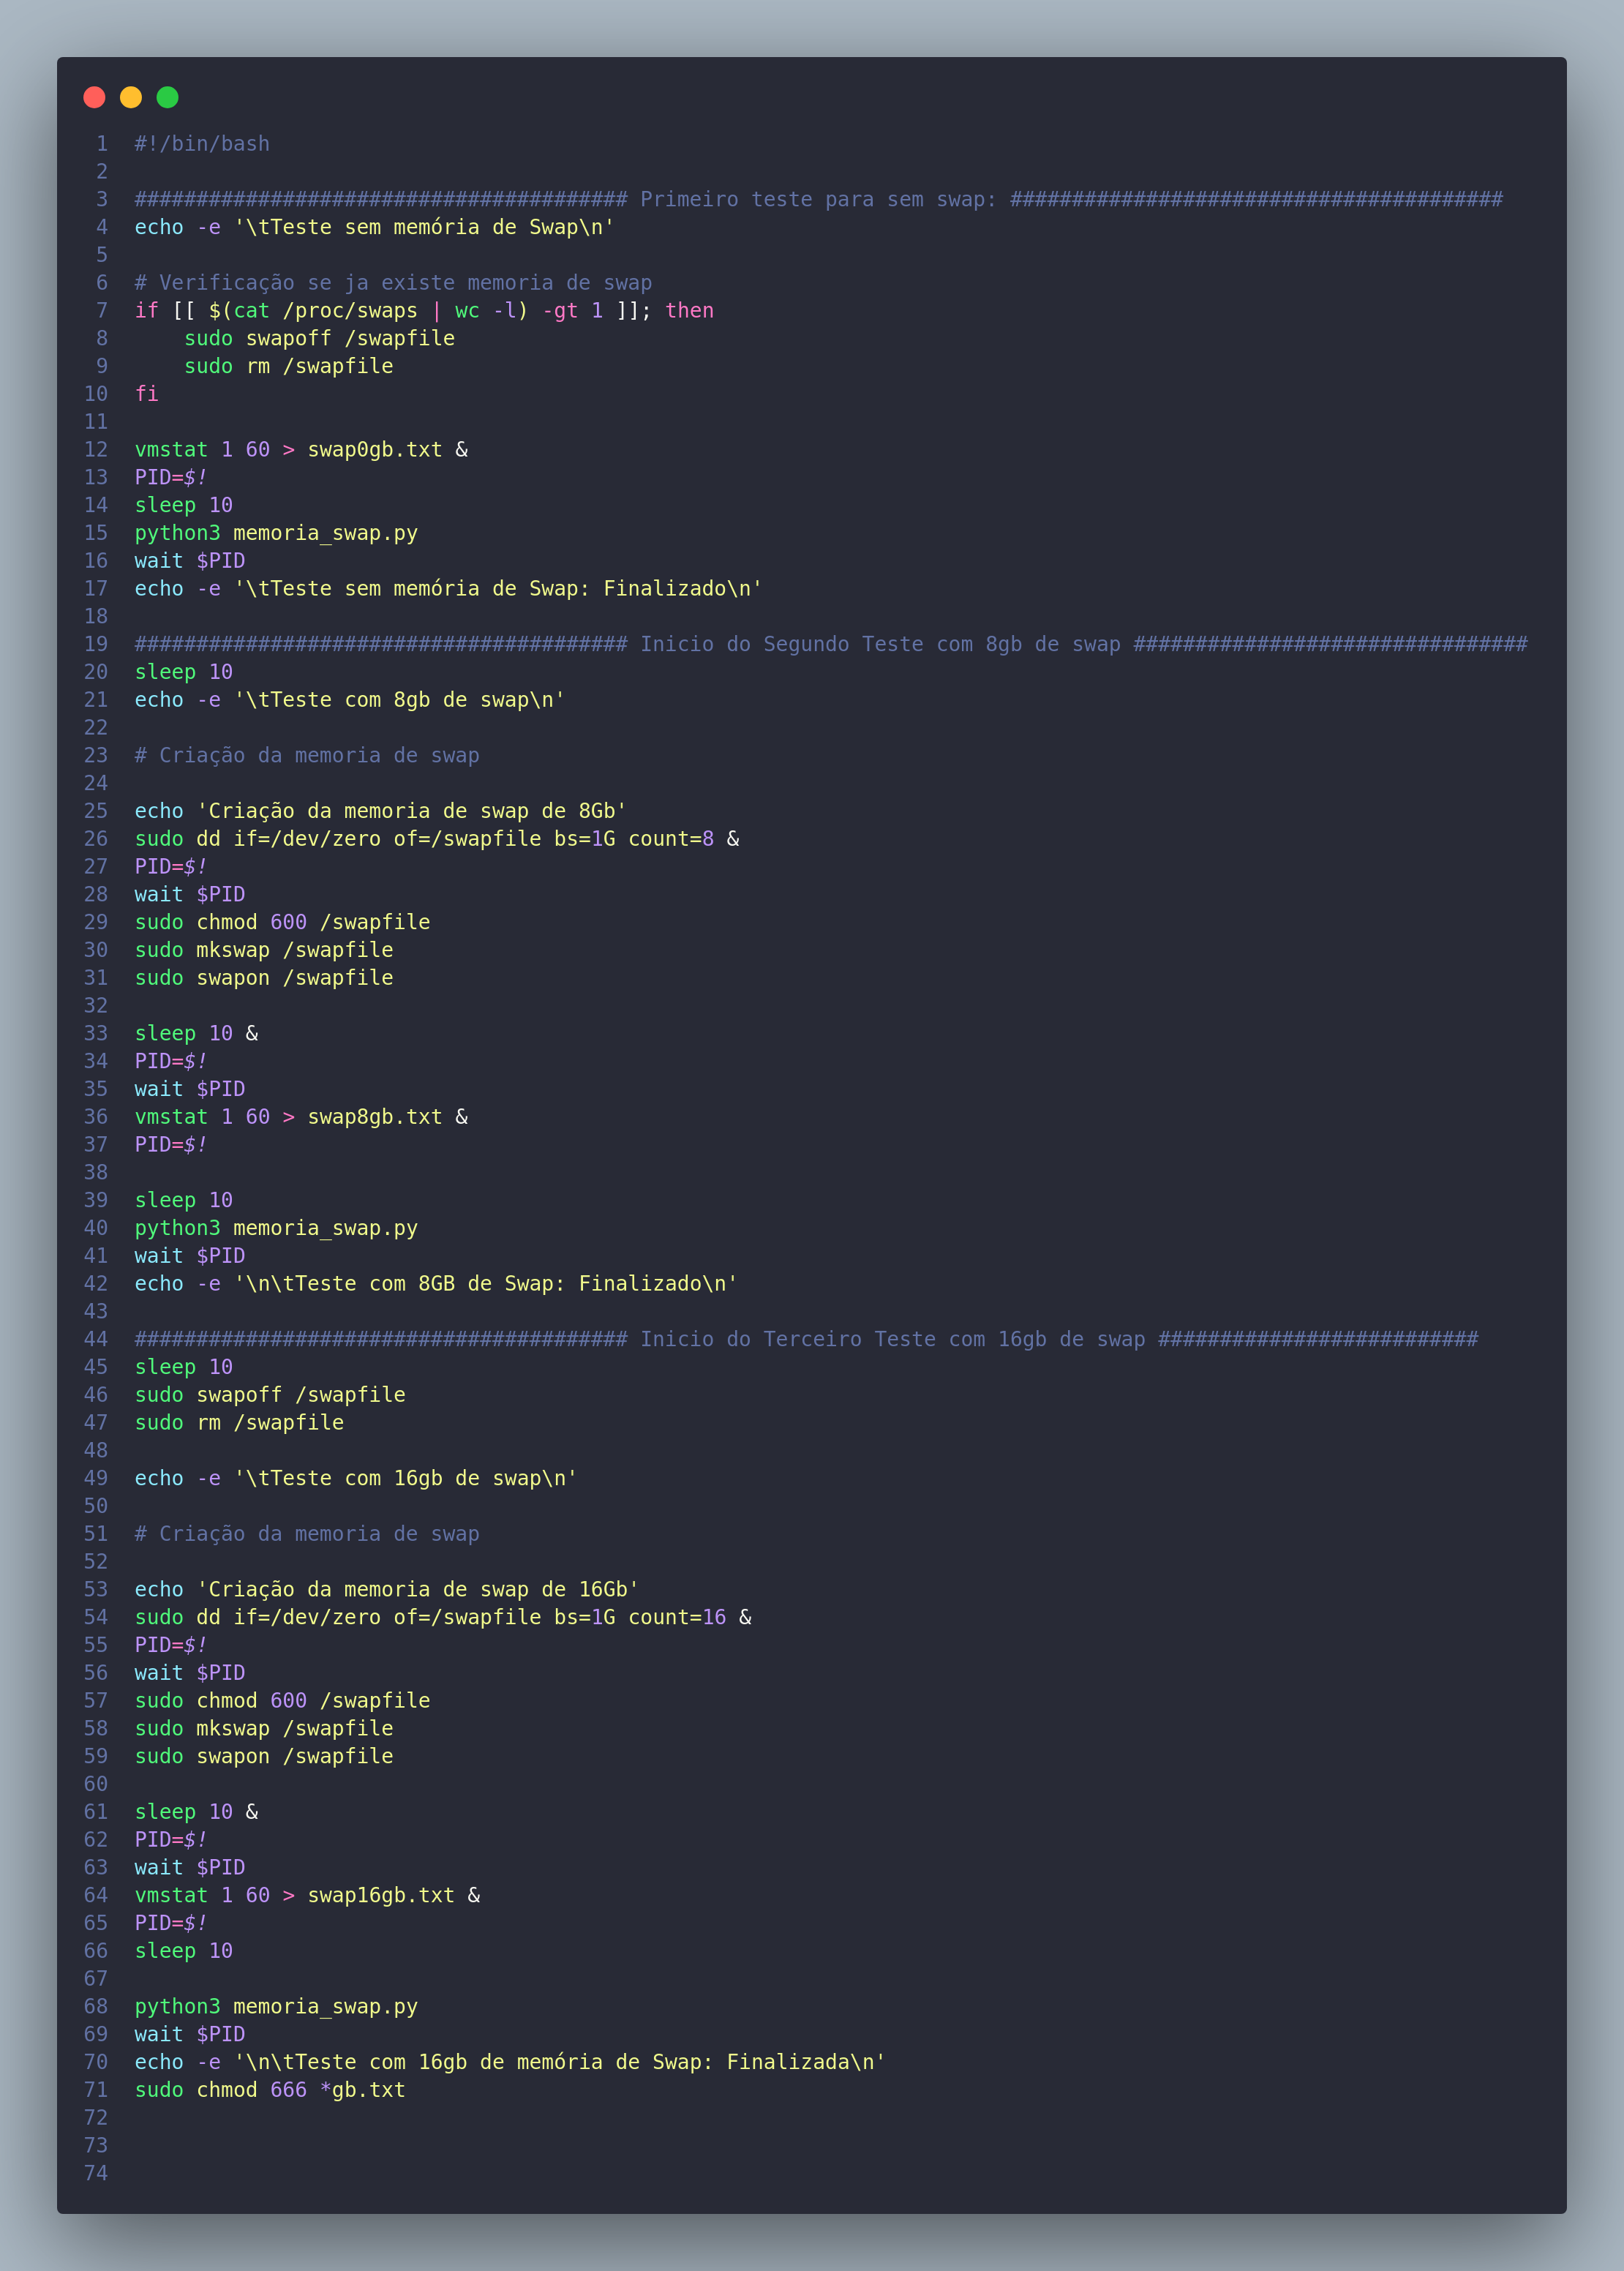
\includegraphics[width=1.0\textwidth]{bash.png}
	\caption{Script em Bash. Disponível em \href{https://github.com/jvictorferreira3301/Sistemas_Operacionais/blob/main/5_swap/swap.sh}{github.com/jvictorferreira3301/SistemasOperacionais
	/blob/main/5\_swap/swap.sh}}
	\label{fig:swapy}
\end{figure}


Abaixo está uma explicação detalhada das principais etapas do script:


\begin{enumerate}[label=\arabic*.]
    \item \textbf{Teste sem memória de Swap:}
    \begin{itemize}
        \item Verifica se há alguma partição de swap ativa e a desativa, se existir.
        \item Inicia a coleta de estatísticas do sistema usando o comando \texttt{vmstat 1 60} e redireciona a saída para \texttt{swap0gb.txt}.
        \item Inicia a execução do código em Python desenvolvido \texttt{memoria\_swap.py} (\ref{fig:swapy})  após uma pausa de 10 segundos.
        \item Aguarda a conclusão do \texttt{memoria\_swap.py} (\ref{fig:swapy}) antes de encerrar a coleta de estatísticas.
    \end{itemize}

    \item \textbf{Teste com 8GB de Swap:}
    \begin{itemize}
        \item Cria um arquivo de \textit{swap} (\texttt{/swapfile}) com tamanho de 8GB.
        \item Atribui permissões adequadas ao arquivo de \textit{swap}.
        \item Formata o arquivo de \textit{swap} e ativa o \textit{swap}.
        \item Inicia a coleta de estatísticas do sistema usando \texttt{vmstat 1 60} e redireciona a saída para \texttt{swap8gb.txt}.
        \item Inicia a execução do \texttt{memoria\_swap.py} (\ref{fig:swapy}) após uma pausa de 10 segundos.
        \item Aguarda a conclusão do \texttt{memoria\_swap.py} (\ref{fig:swapy}) antes de encerrar a coleta de estatísticas.
    \end{itemize}

    \item \textbf{Teste com 16GB de Swap:}
    \begin{itemize}
        \item Desativa e remove o \textit{swap} existente, se houver.
        \item Cria um novo arquivo de \textit{swap} de 16GB.
        \item Atribui permissões adequadas ao novo arquivo de \textit{swap}.
        \item Formata o novo arquivo de \textit{swap} e ativa o \textit{swap}.
        \item Inicia a coleta de estatísticas do sistema usando \texttt{vmstat 1 60} e redireciona a saída para \texttt{swap16gb.txt}.
        \item Inicia a execução do \texttt{memoria\_swap.py} (\ref{fig:swapy}) após uma pausa de 10 segundos.
        \item Aguarda a conclusão do \texttt{memoria\_swap.py} (\ref{fig:swapy}) antes de encerrar a coleta de estatísticas.
    \end{itemize}
\end{enumerate}

Ao final de cada teste, o script ajusta as permissões dos arquivos de saída (\texttt{swap0gb.txt}, 
\texttt{swap8gb.txt}, \texttt{swap16gb.txt}) para permitir o acesso. Os resultados desses testes 
fornecem informações sobre o impacto da configuração da memória de troca no desempenho do sistema 
em um ambiente Linux.

Como descrito, nesses arquivos de texto citados são gravadas estatísticas oriundas do \texttt{vmstat}, porém nem todas 
as estatísticas gravadas são interessantes, então, utilizando a biblioteca pandas do Python, foi feito um tratamento 
nos dados para que fossem mostradas, em um dataframe, somente as seguintes informações:

\begin{itemize}
    \item \textbf{swpd (Swap Used):} Indica a quantidade de espaço de swap que está atualmente em uso no sistema. Valores não nulos indicam que o sistema está fazendo uso do swap.

    \item \textbf{si (Swap In):} Indica a quantidade de dados sendo movida do disco para a memória swap (swap in). Um aumento em `si` significa que o sistema está transferindo dados do swap de volta para a memória principal.

    \item \textbf{so (Swap Out):} Indica a quantidade de dados sendo movida da memória para o disco swap (swap out). Um aumento em `so` significa que o sistema está transferindo dados da memória principal para o swap.

    \item \textbf{us (CPU User Time):} Porcentagem de tempo da CPU gasto na execução de código de usuário. Se o swap estiver sendo usado intensivamente, pode haver um aumento na carga da CPU.

    \item \textbf{sy (CPU System Time):} Porcentagem de tempo da CPU gasto no kernel (sistema). Se o sistema estiver movendo dados entre a memória e o swap, isso pode refletir no tempo do sistema.
\end{itemize}

Os resultados dos 3 cenários (\ref{chap:des}) com as informações acima podem ser vistos nas seguintes tabelas:

\begin{figure}[H]
	\centering
	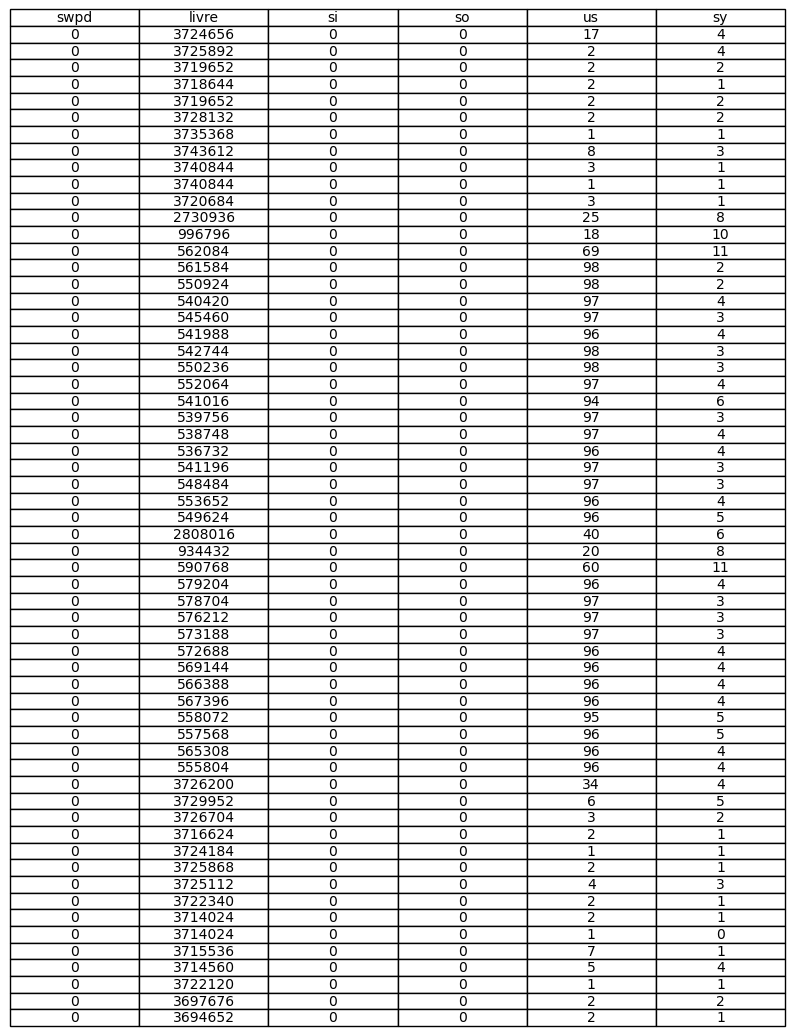
\includegraphics[width=1.0\textwidth]{swap0gb.png}
	\caption{Resultados do teste sem Swap (0gb)}
	\label{fig:swap0}
\end{figure}

\begin{figure}[H]
	\centering
	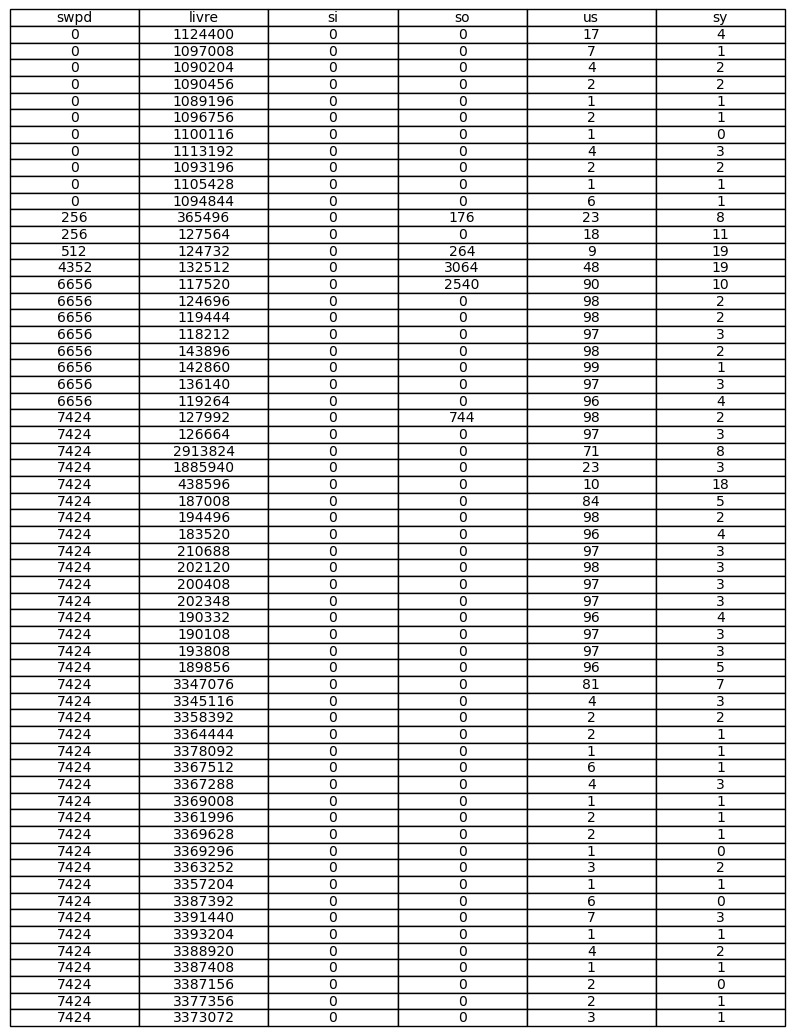
\includegraphics[width=1.0\textwidth]{swap8gb.png}
	\caption{Resultados do teste com Swap igual a RAM (8gb)}
	\label{fig:swap8}
\end{figure}

\begin{figure}[H]
	\centering
	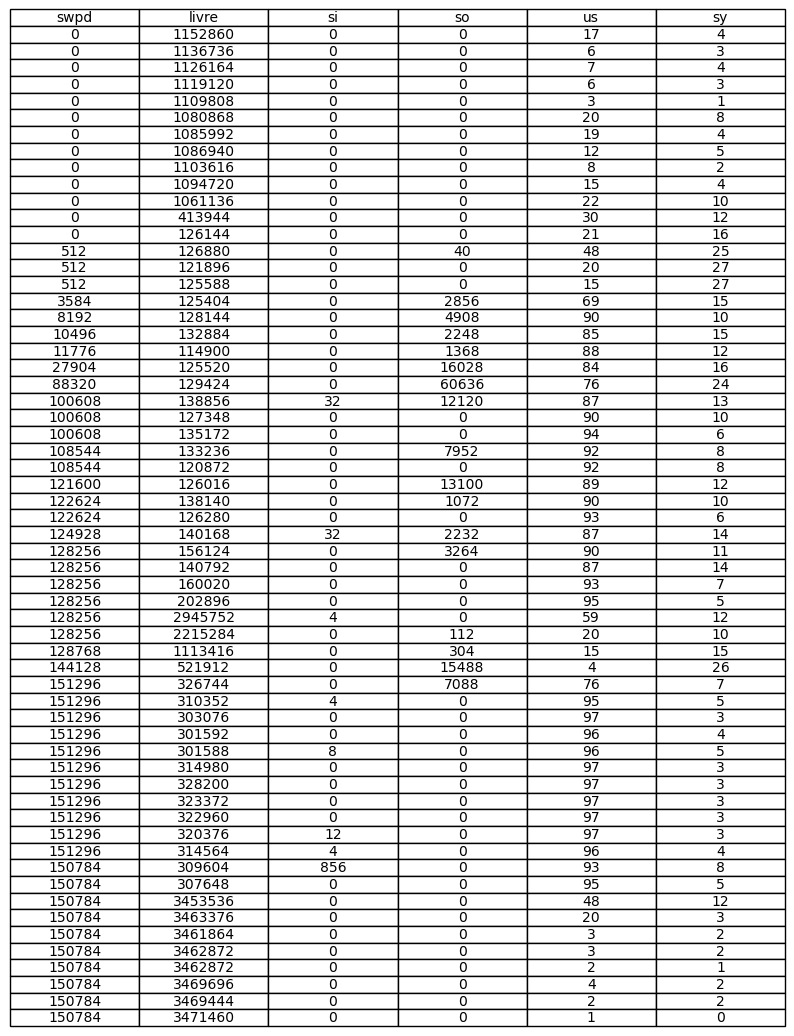
\includegraphics[width=1.0\textwidth]{swap16gb.png}
	\caption{Resultados do teste com Swap duas vezes maior que a RAM (16gb)}
	\label{fig:swap16}
\end{figure}

Essas tabelas foram obtidas através de um script em Jupyter Notebook que pode ser acessado 
\href{https://github.com/jvictorferreira3301/Sistemas_Operacionais/blob/main/5_swap/swap.sh}{clicando aqui} 
e os arquivos de texto brutos sem o tratamento podem ser vistos em  \href{https://github.com/jvictorferreira3301/Sistemas_Operacionais/blob/main/5_swap}{github.com/jvictorferreira3301/SistemasOperacionais
/blob/main/5\_swap}.

\section{Análise Comparativa dos 3 Cenários de Swap}
\subsection{Sem Swap (0gb)}
Testar um cenário sem memória de swap é crucial para compreender o comportamento do sistema quando a RAM atinge sua capacidade máxima. 
Isso permite a avaliação comparativa do desempenho entre diferentes configurações de tamanho de memória de swap. Ao simular a ausência de memória de troca,
é possível analisar como o sistema se comporta em situações de alta demanda de memória, identificar quais configurações de swap podem ser mais
eficazes e compreender o impacto da presença ou ausência de memória de troca no desempenho do sistema em várias cargas de trabalho.

\begin{figure}[H]
	\centering
	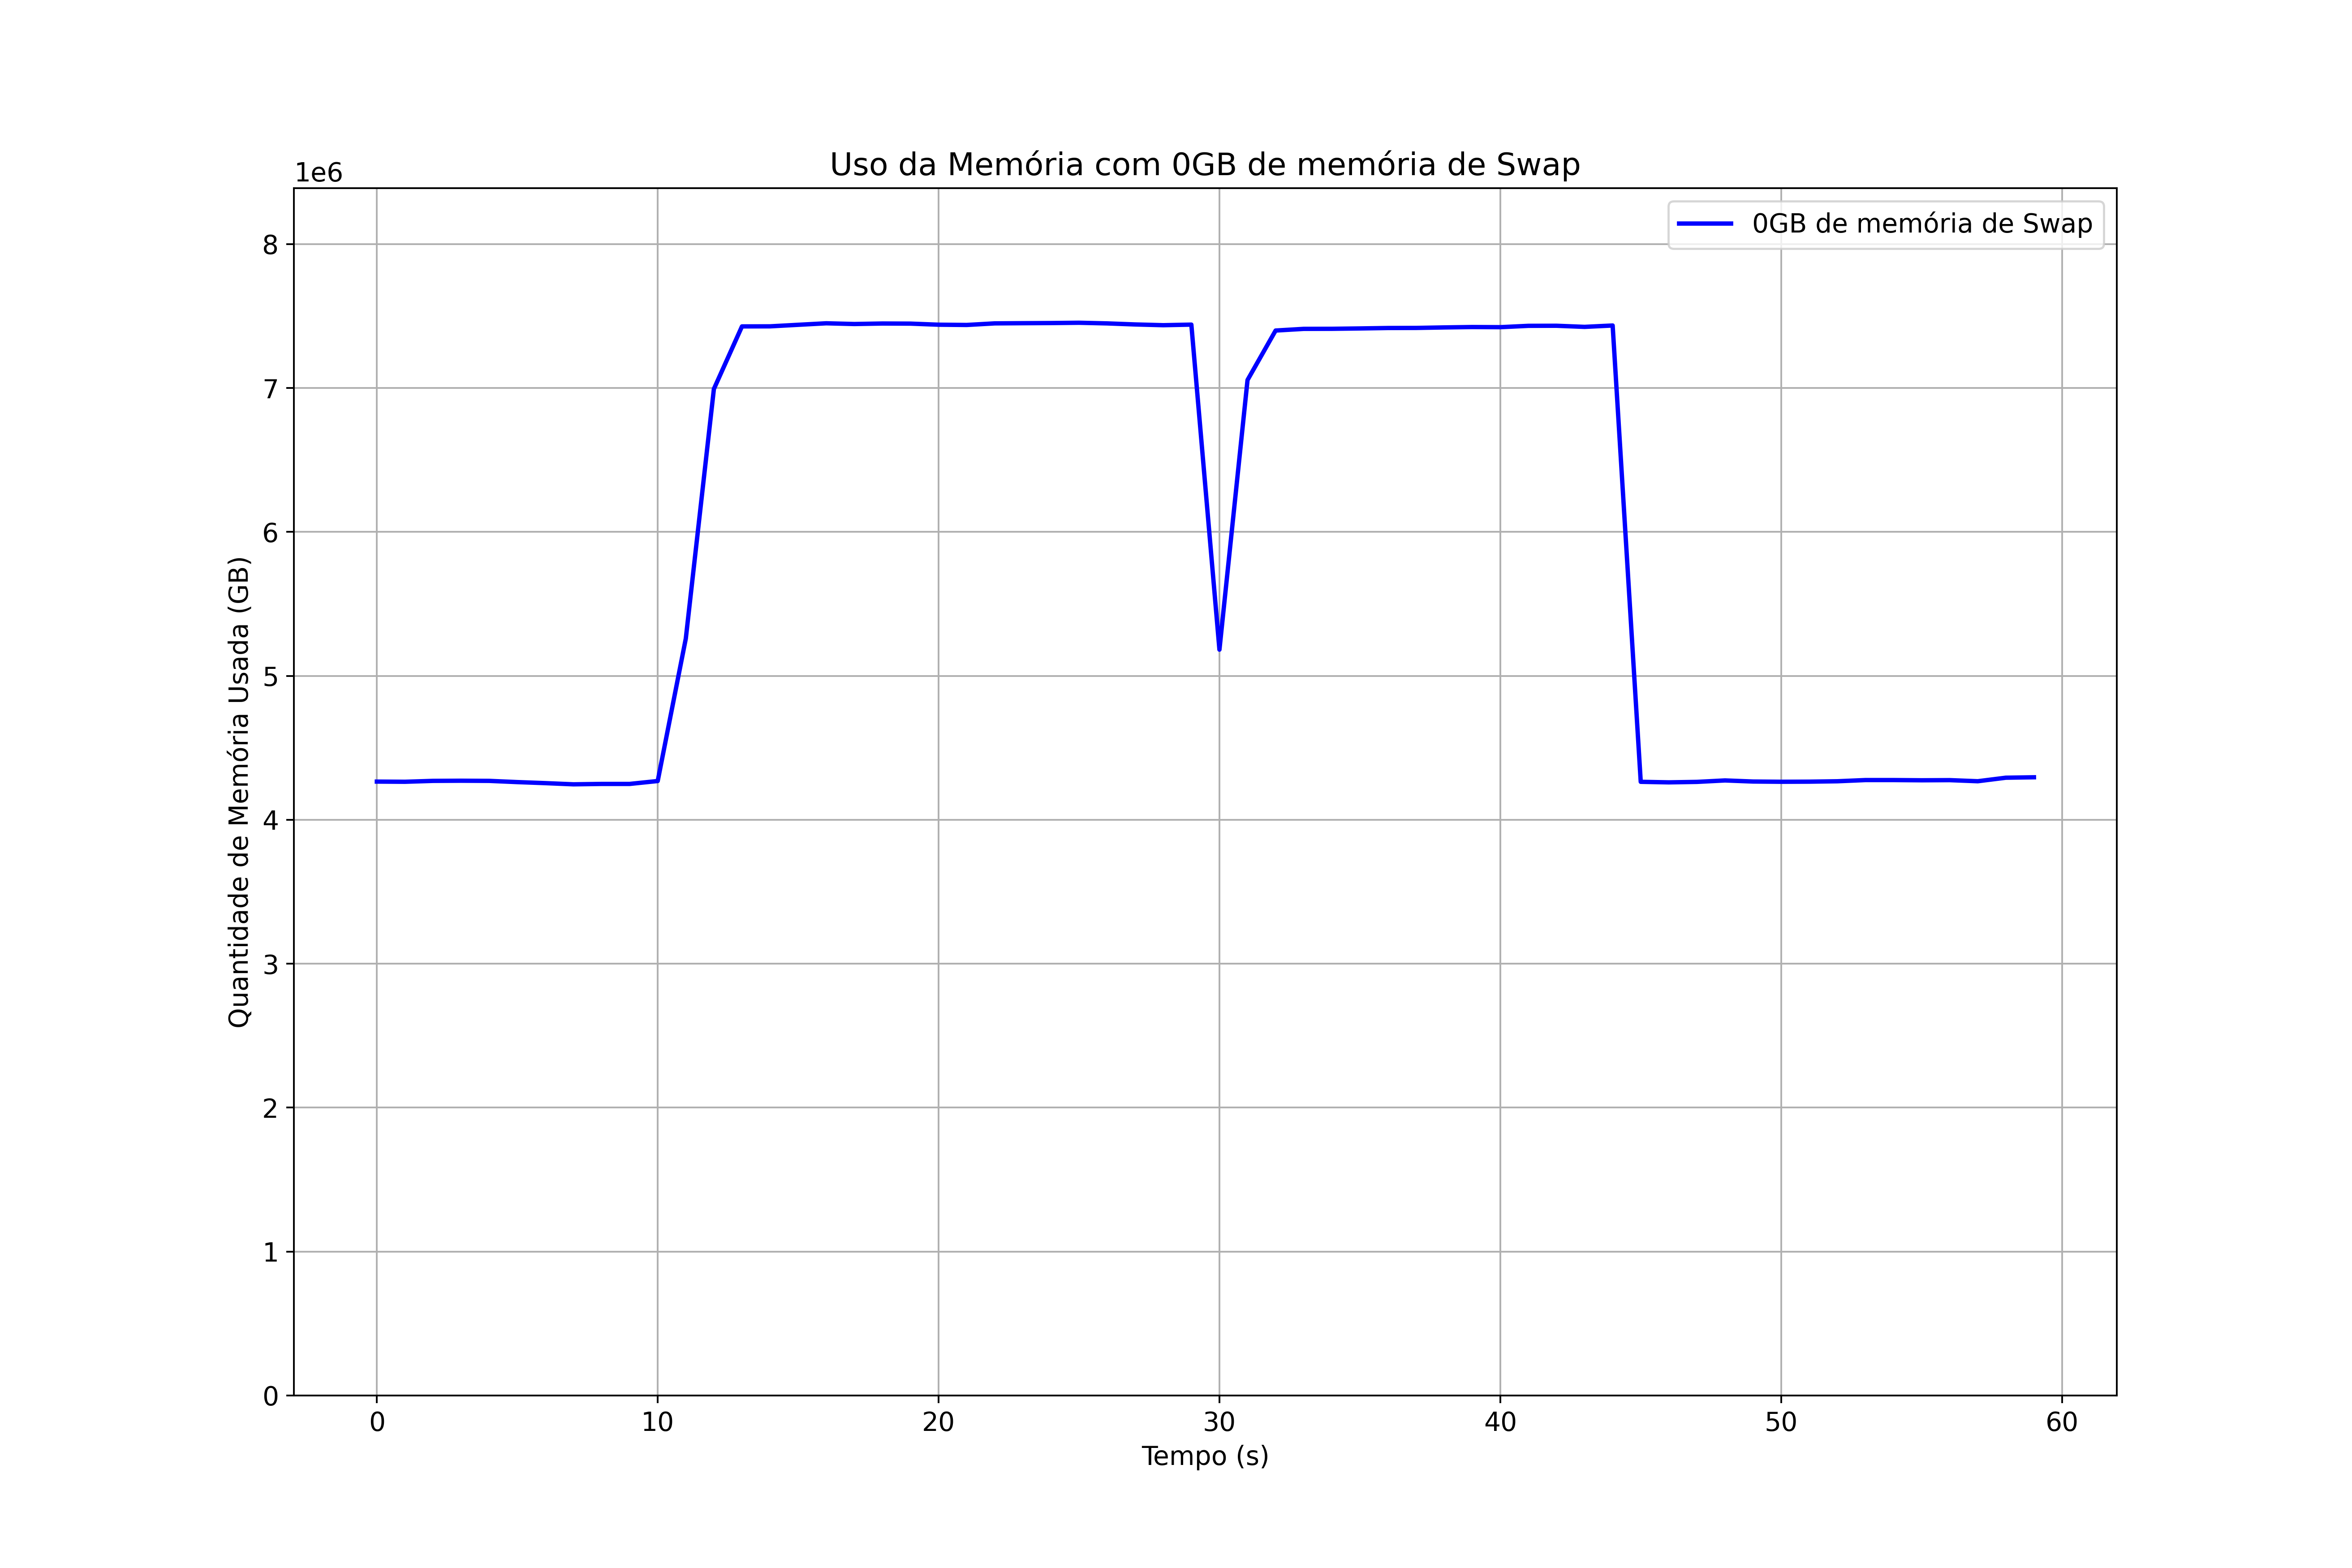
\includegraphics[width=1.0\textwidth]{0gb_swap.png}
	\caption{Uso da mémoria com 0GB de mémoria de Swap}
	\label{fig:testes_swap0}
\end{figure}

A figura \ref{fig:testes_swap0} representa a alocação dinâmica de memória durante a execução do código de teste. No gráfico, o eixo horizontal 
representa o tempo em segundos, mostrando a evolução da execução do teste. O eixo vertical representa o uso de memória 
em gigabytes (GB), oferecendo uma visão do consumo de recursos ao longo do tempo. Durante um intervalo específico de tempo, entre 
t = 10s e t = 45s, observa-se que o uso de memória atingiu e se manteve no nível máximo disponível no sistema. Esse período de 35
segundos é marcado por um consumo constante de memória, refletindo a capacidade máxima do computador sendo plenamente utilizada.

\subsection{Swap Igual à RAM (8gb):}
Nesse novo contexto, o aumento da quantidade de memória de swap para 8GB levanta a expectativa de que programas com demandas mais elevadas 
de memória possam apresentar maior agilidade. Isso se deve à ampliação da capacidade de armazenamento temporário oferecida
pela memória de swap. Com essa extensão adicional, prevê-se que o sistema possa lidar de forma mais eficaz com operações que 
demandam grandes recursos de memória, reduzindo possíveis interrupções ou atrasos ocasionados pela limitação do espaço de memória.

\begin{figure}[H]
	\centering
	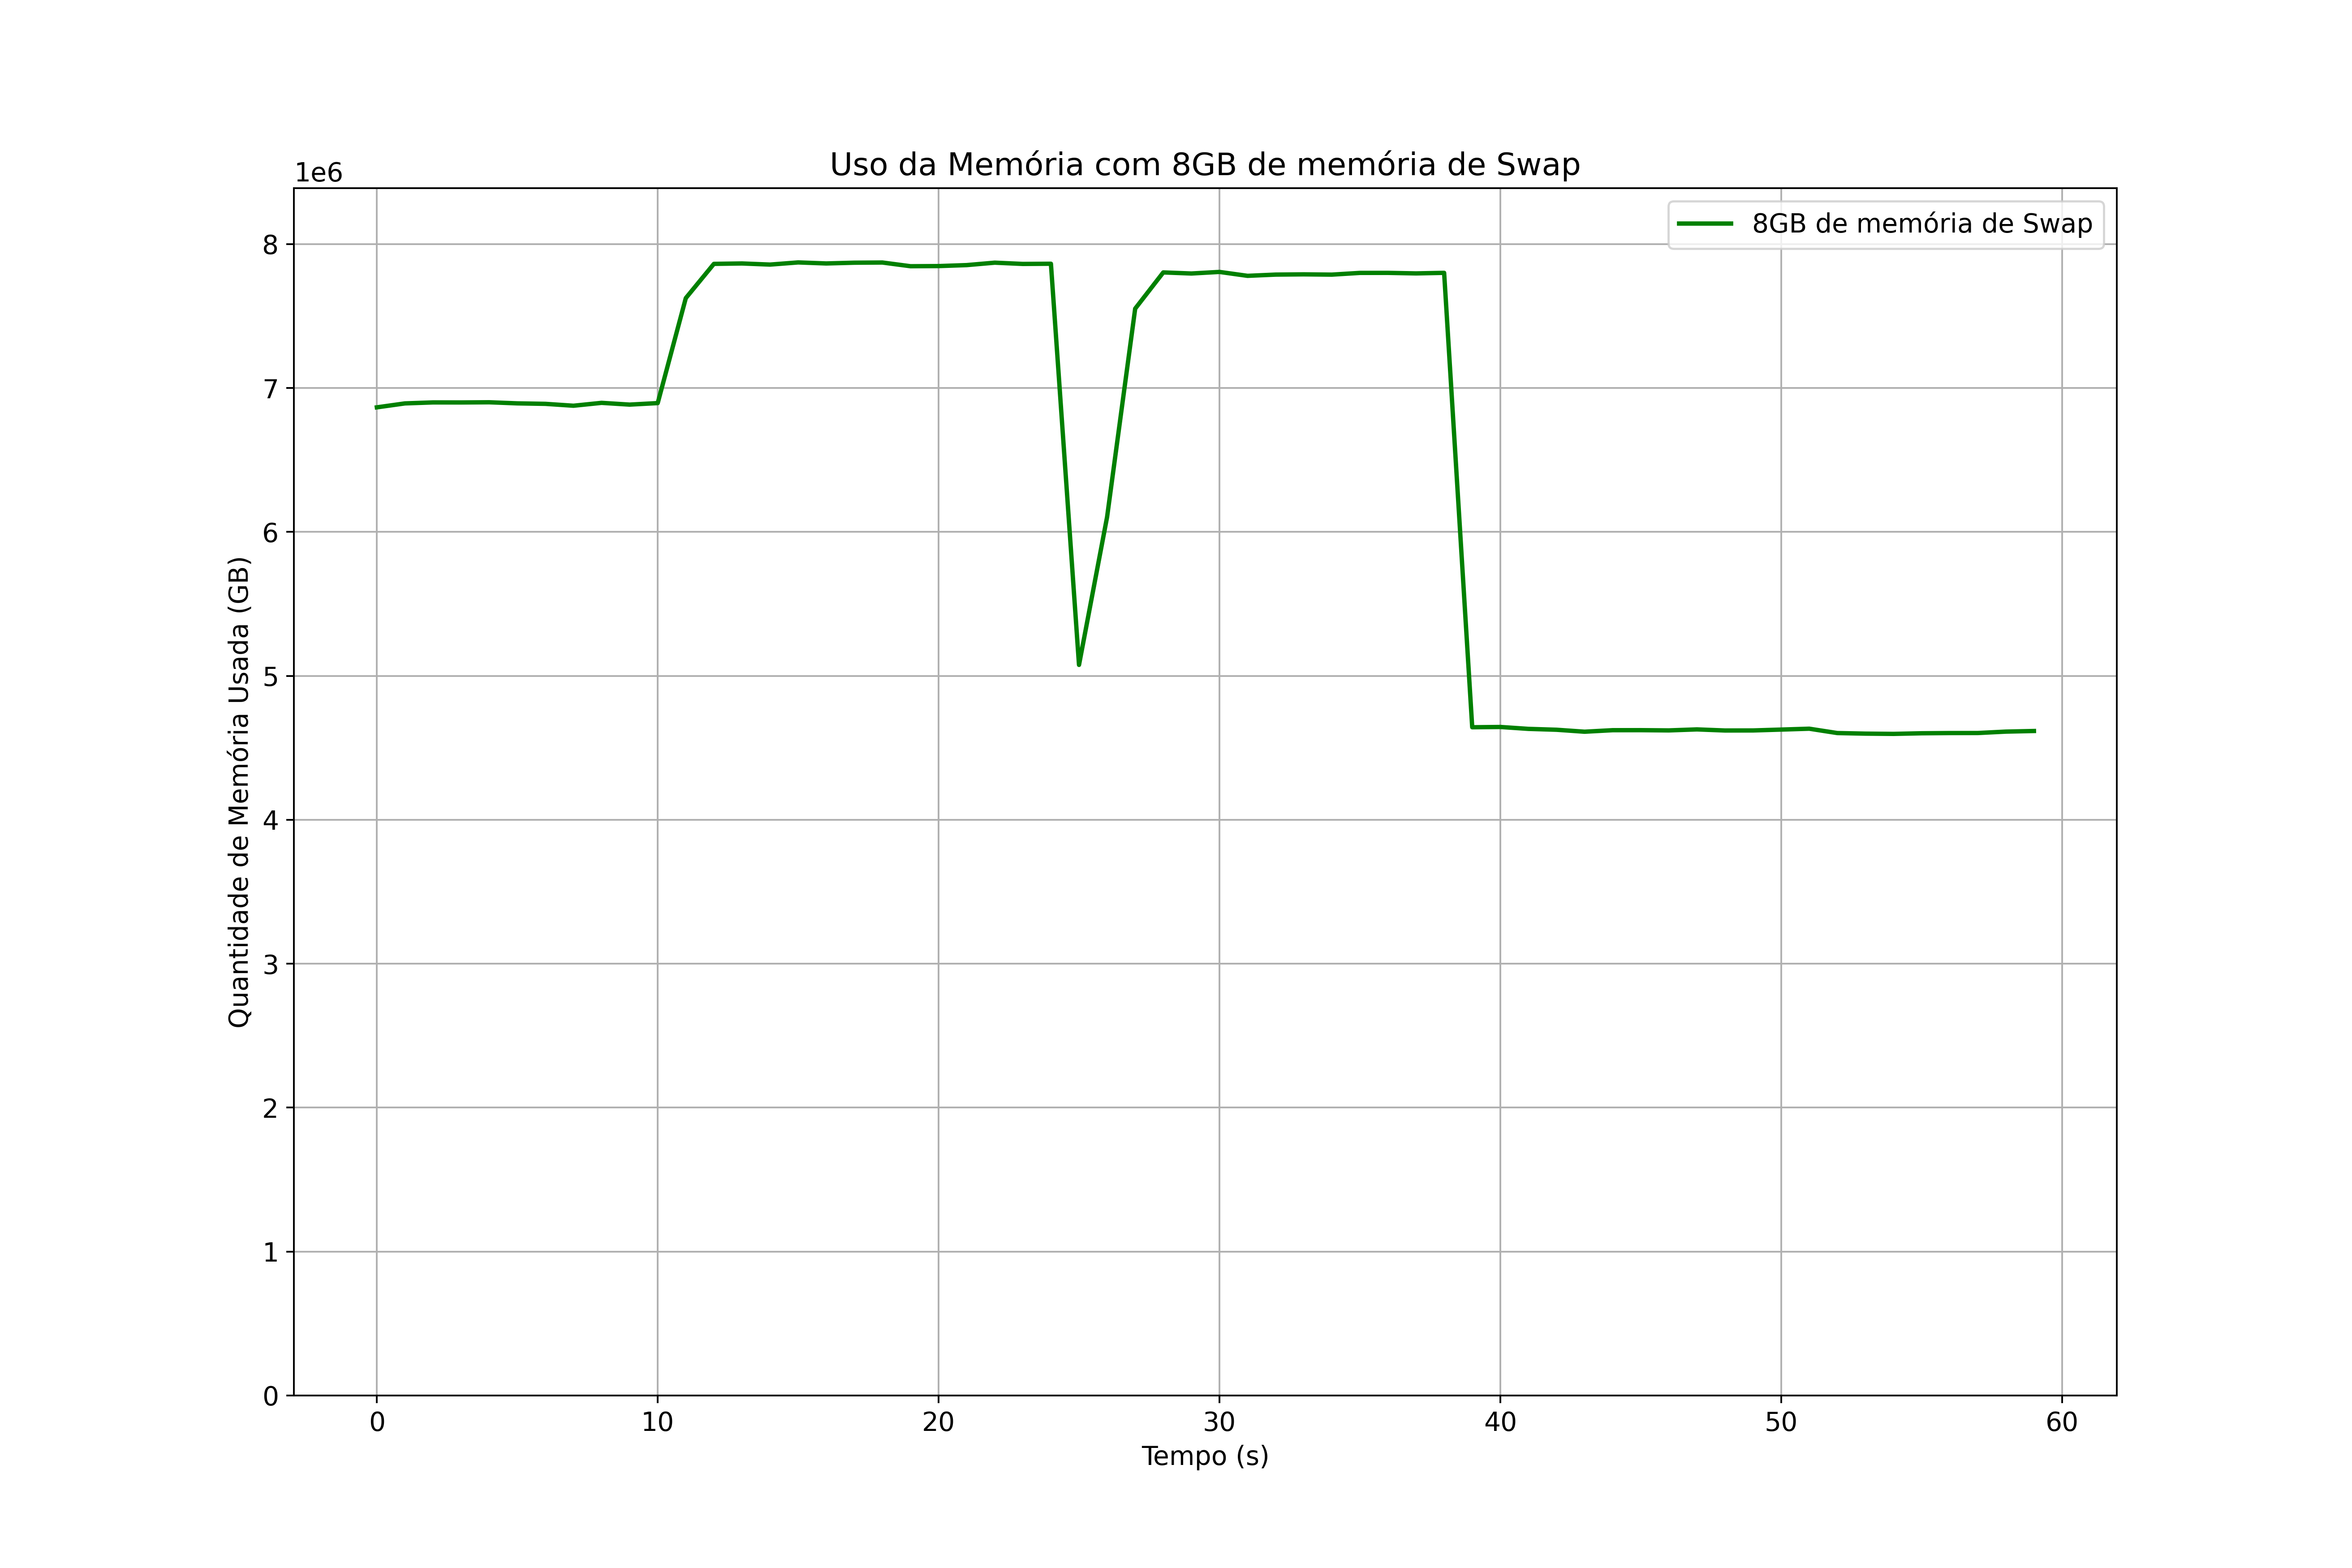
\includegraphics[width=1.0\textwidth]{8gb_swap.png}
	\caption{Uso da mémoria com 8GB de mémoria de Swap}
	\label{fig:testes_swap8}
\end{figure}

A figura \ref{fig:testes_swap8} representa a alocação dinâmica de memória durante a execução do código de teste. No gráfico, o eixo
horizontal representa o tempo em segundos, mostrando a evolução da execução do teste. O eixo vertical represneta o uso de mémoria
em gigabytes (GB). Durante um intervalo de tempo específico, entre t = 10s e t = 39s, observa-se que o uso de mémoria atingiu e se
manteve no nível máximo disponível no sistema por 29 segundos. Essa otimização é esperada devido ao aumento da quantidade de 
memória de swap para 8GB

\subsection{Swap duas vezes maior que a RAM (16gb):}
Uma questão relevante a ser considerada é se a utilização de memória de swap auxilia na otimização do gerenciamento de memória. Surge 
a questão sobre a viabilidade de aumentar indefinidamente a memória de swap, dada a possibilidade de melhoria na alocação de 
recursos. Este teste foi elaborado para investigar se um aumento significativo na memória de swap resulta de fato em melhorias 
mensuráveis no desempenho do sistema, explorando os limites dos benefícios proporcionados pela expansão da memória de swap.

\begin{figure}[H]
	\centering
	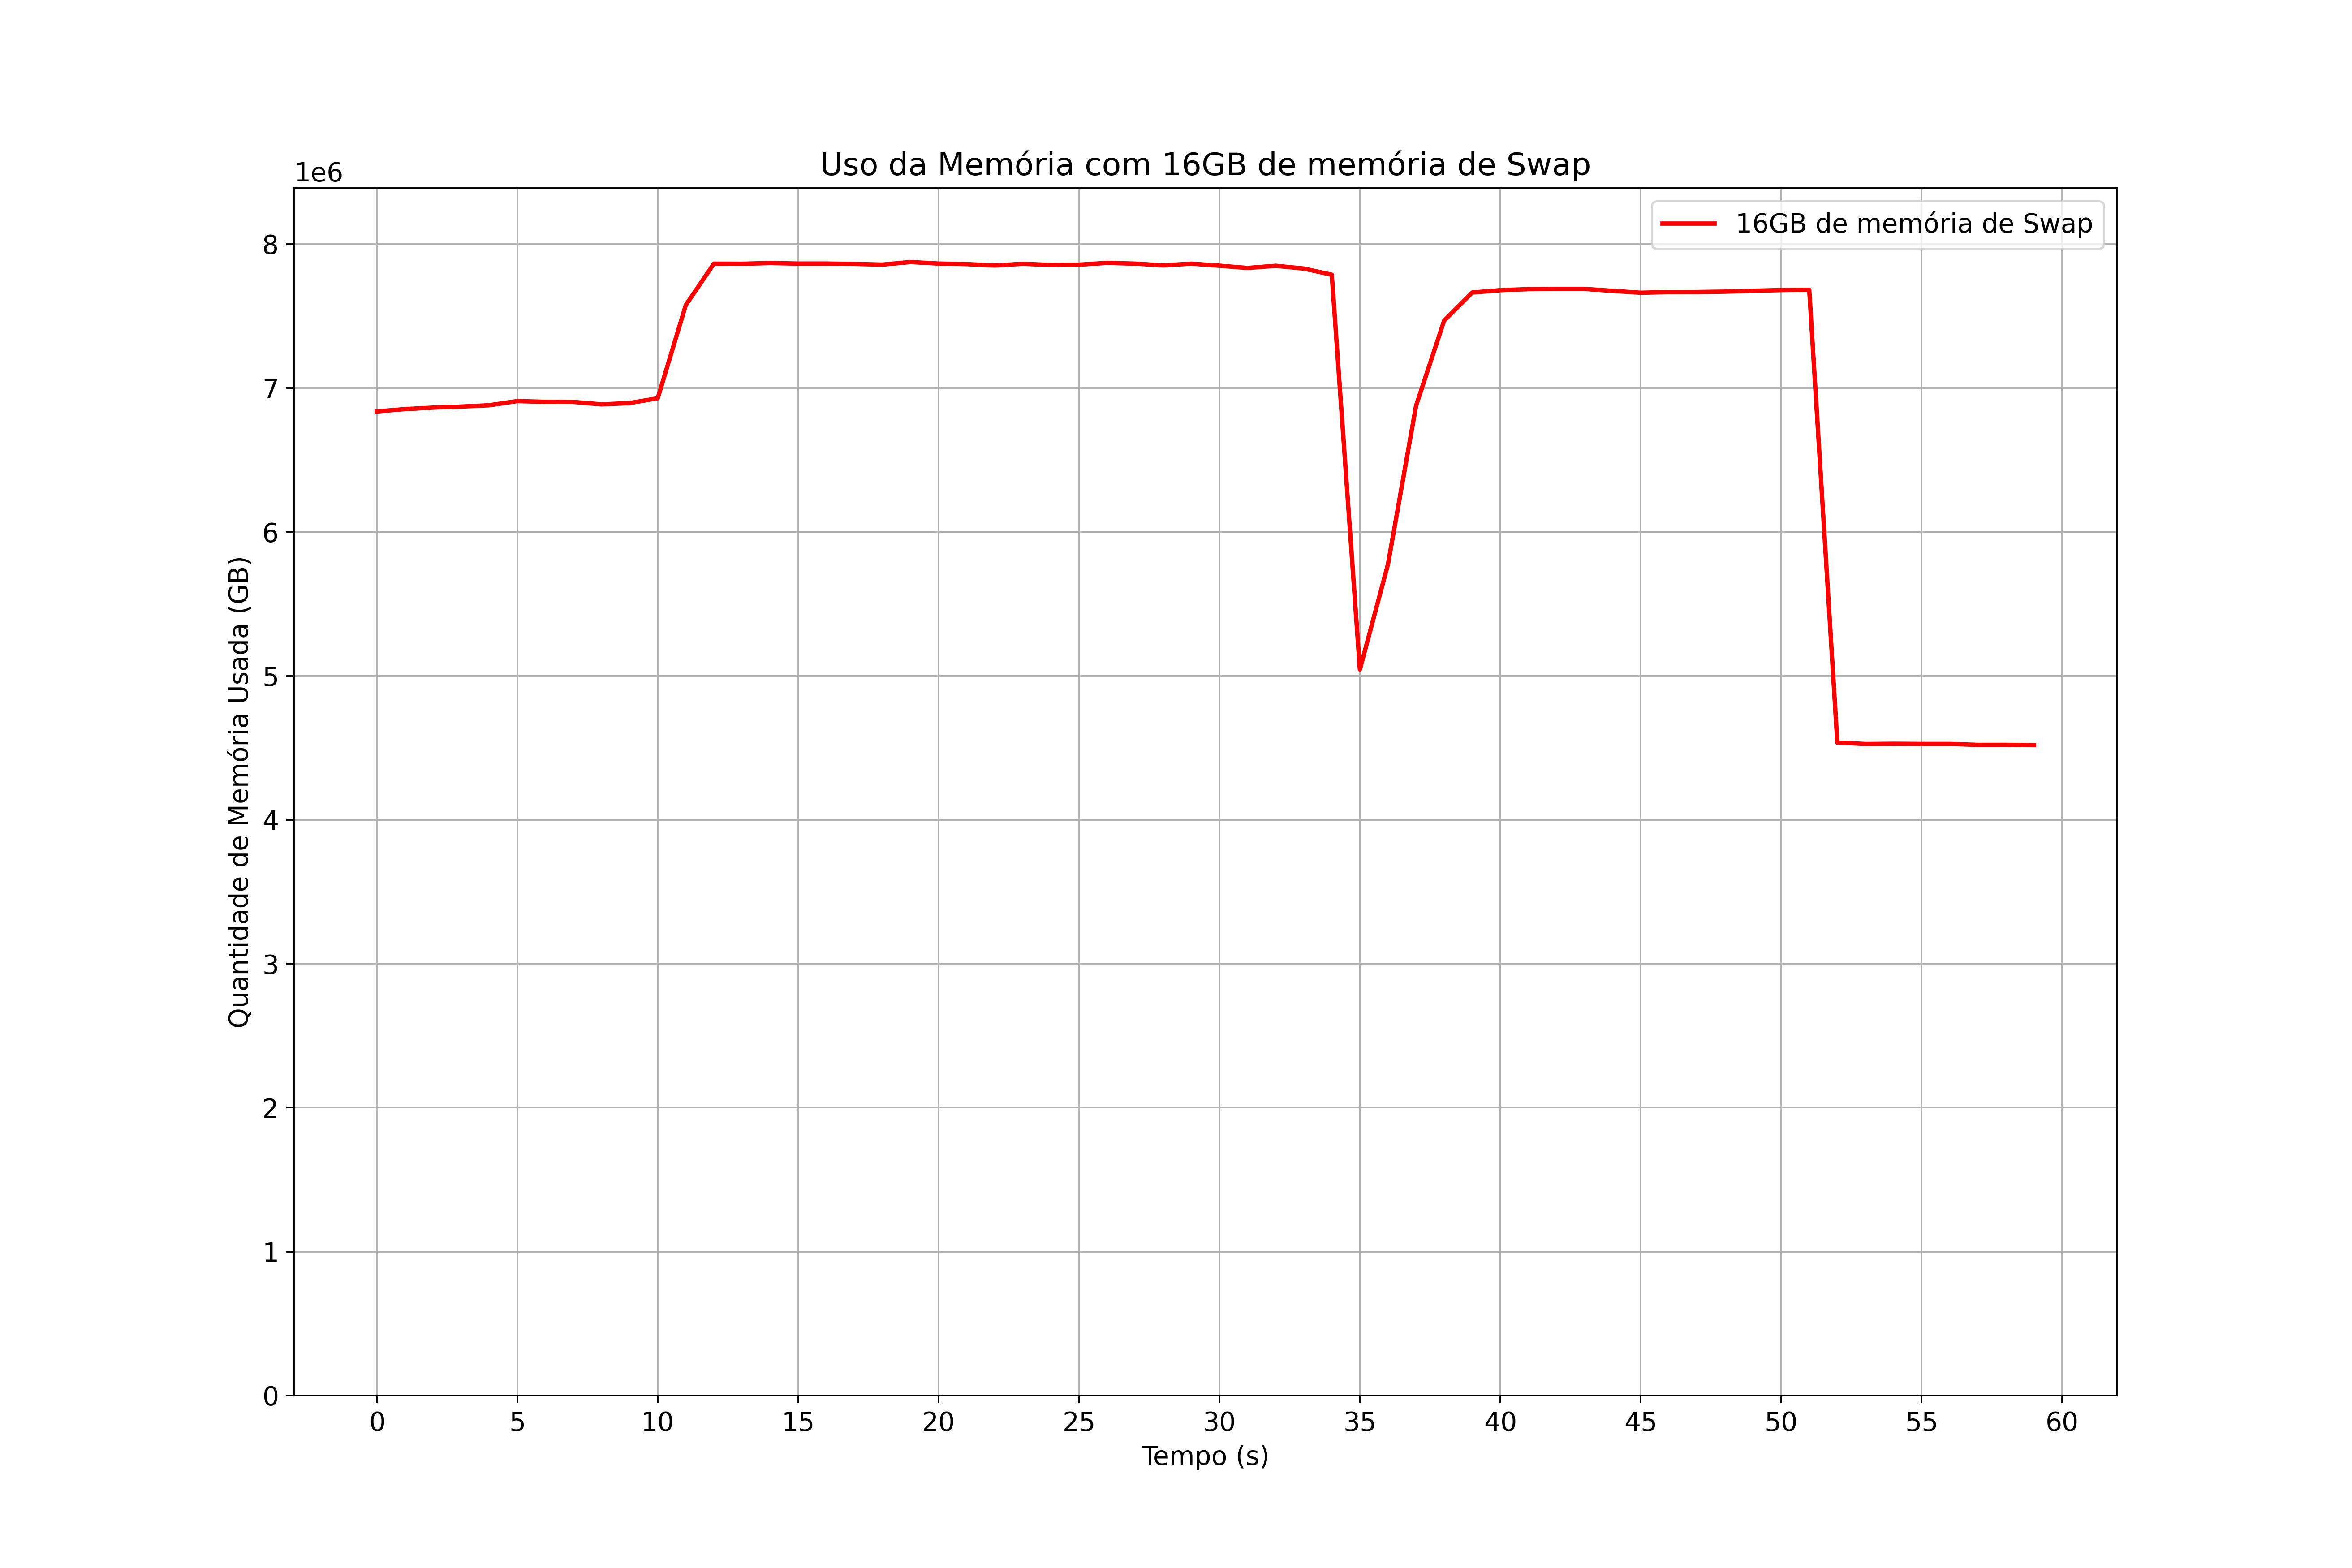
\includegraphics[width=1.0\textwidth]{16gb_swap.png}
	\caption{Uso da mémoria com 16GB de mémoria de Swap}
	\label{fig:testes_swap16}
\end{figure}

A figura \ref{fig:testes_swap16} representa a alocação dinâmica de memória durante a execução do código de teste. No gráfico, o eixo
horizontal representa o tempo em segundos, mostrando a evolução da execução do teste. O eixo vertical represneta o uso de mémoria
em gigabytes (GB). Durante um intervalo de tempo específico, entre t = 10s e t = 52s, observa-se que o uso de mémoria atingiu e se
manteve no nível máximo disponível no sistema por 42 segundos.

\section{Considerações Importantes para o Benchmark}
Ao analisar o desempenho do sistema operacional com a memória de Swap, é crucial levar em 
consideração vários fatores que podem influenciar os resultados, como o hardware em que os testes foram realizados.


O desempenho da memória de swap é profundamente influenciado pelo hardware subjacente. Elementos como a natureza e a 
velocidade do dispositivo de armazenamento utilizado para a memória de troca, seja um disco rígido (HDD) ou um disco de estado sólido 
(SSD), bem como suas configurações específicas, a quantidade e a velocidade da memória RAM disponível no sistema, e a capacidade do 
processador (CPU), desempenham papéis cruciais nos resultados obtidos em testes de desempenho da memória de swap. Esses atributos do 
hardware são determinantes na eficácia e na velocidade de acesso aos dados armazenados na memória de swap, influenciando diretamente 
a capacidade do sistema em lidar eficientemente com a troca de informações entre a memória principal e o armazenamento secundário.
Em nossa análise foi usado uma máquina com as características especificadas na tabela \ref{tab:ideapad_specs}


\begin{table}[H]
    \centering
    \caption{Especificações do Hardware usado}
    \begin{tabular}{@{}ll@{}}
        \toprule
        \textbf{Componente} & \textbf{Especificação} \\
        \midrule
        Processador & Intel Core i5-7400 \\
        Memória RAM & 8 GB DDR4 (1x8) 2666 \\
        Armazenamento & SSD SATA 480 GB \\
        Sistema Operacional & Ubuntu 22.04 LTS \\
        \bottomrule
    \end{tabular}
    \label{tab:ideapad_specs}
\end{table}


\chapter{Conclusão}
\label{conclusao}

A criação da memória de swap teve como propósito primordial mitigar as restrições inerentes à capacidade física da memória RAM, objetivando minimizar os 
incidentes relacionados à insuficiência de memória e otimizar o funcionamento do sistema. Nesse contexto, é crucial analisar cuidadosamente
se a ampliação substancial da memória de swap é uma medida vantajosa e justificável, dado o potencial impacto na performance do sistema.

\begin{figure}[H]
	\centering
	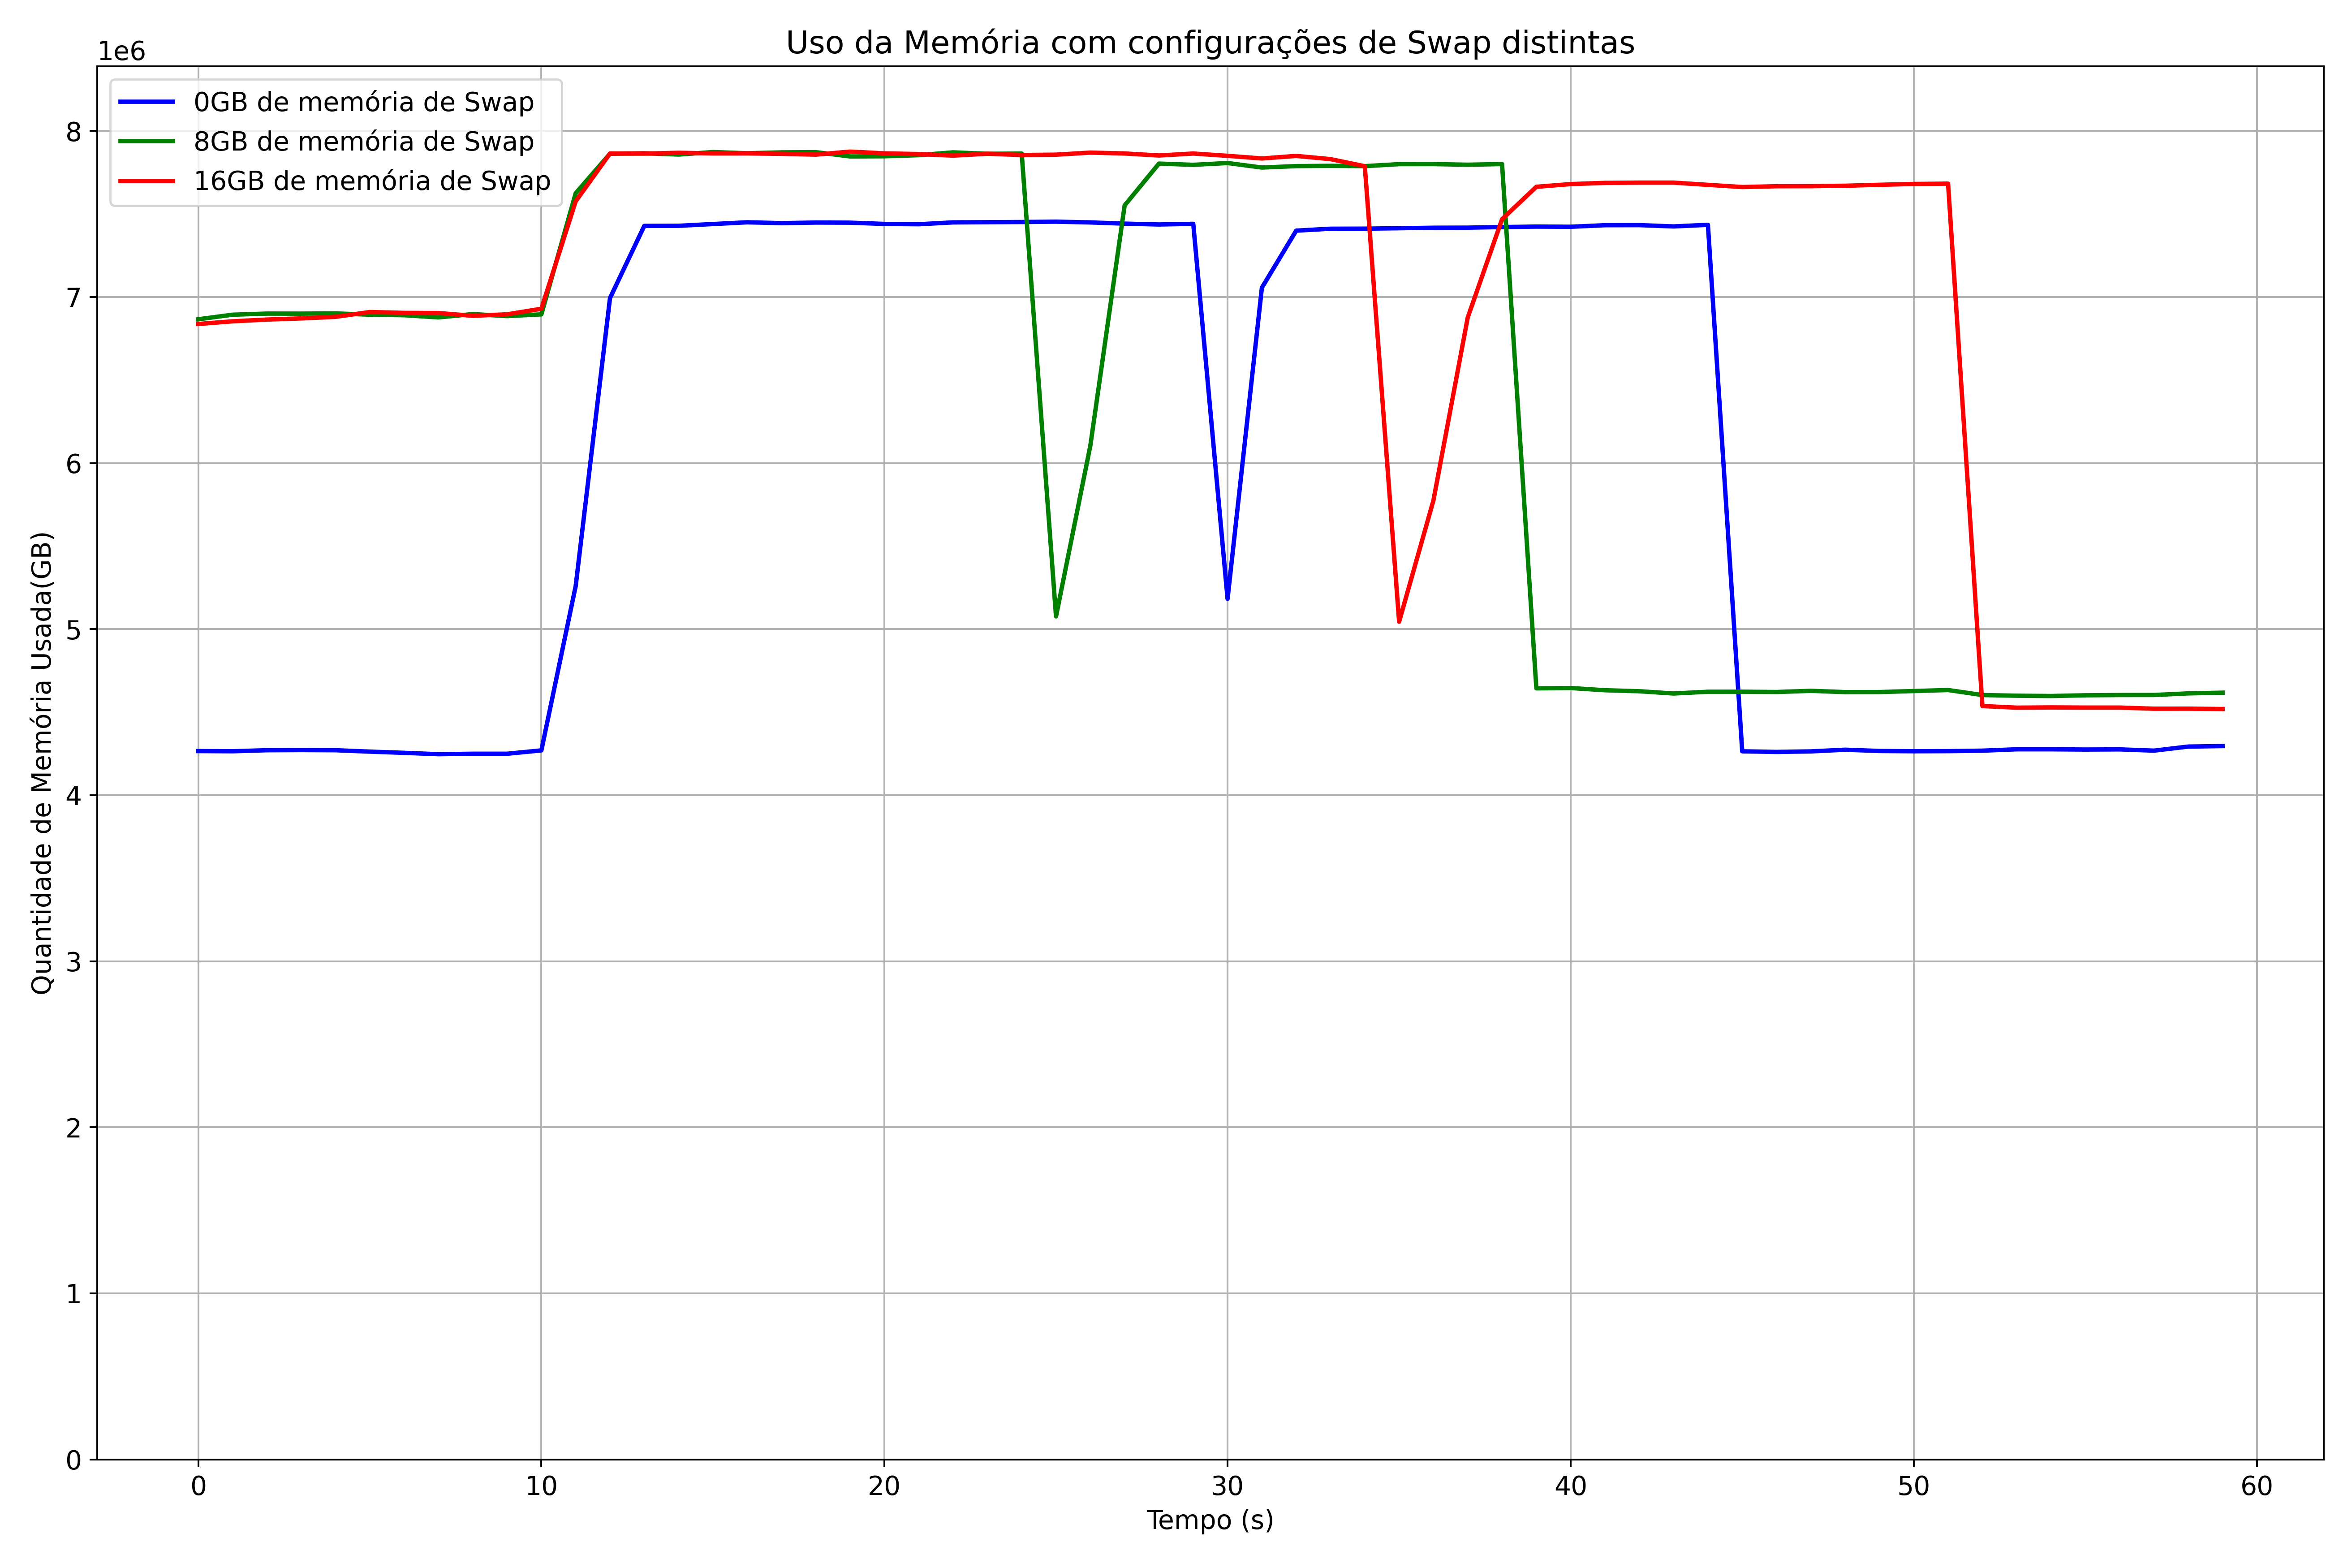
\includegraphics[width=1.0\textwidth]{comparar.png}
	\caption{Comparação do uso de memória}
	\label{fig:comparacao_memoria}
\end{figure}


Na figura \ref{fig:comparacao_memoria}, observa-se que um aumento substancial na capacidade de memória de swap impacta o desempenho do processamento de memória. Notavelmente, quando alocados 
8GB de memória de swap, a execução do código de teste demonstra maior velocidade. Em contraste, ao aumentar para 16 GB de memória de swap, espera-se uma redução no tempo de processamento, 
porém, contrariando a expectativa, o desempenho se degrada.


A degradação do desempenho ao aumentar a capacidade de memória de swap pode ser atribuída a fatores como o gerenciamento excessivo do sistema operacional. Quando a memória de swap é 
ampliada para 16 GB, pode ocorrer um aumento na propensão do sistema em utilizar a troca de memória de maneira mais frequente. Isso pode resultar em operações de transferência entre a
memória principal e a memória de swap, causando um efeito contraproducente ao invés de otimizar a performance.

Além disso, a alocação excessiva de memória de troca pode gerar um impacto negativo devido a possíveis limitações de hardware ou configurações específicas do sistema. Nesse contexto,
o tempo de acesso e manipulação dos dados na memória de troca pode se tornar mais lento do que o acesso direto à memória principal, resultando em um aumento no tempo de processamento, 
mesmo com uma capacidade de troca teoricamente maior.


A presença e o dimensionamento da memória de swap, seja ausente, configurada em 8 GB ou expandida para 16 GB, influenciam significativamente o desempenho do sistema. A ausência de 
memória de swap pode limitar a capacidade de lidar com picos de demanda, levando a uma possível degradação quando a memória física se esgota. Por outro lado, uma alocação moderada, 
como 8 GB, pode otimizar o desempenho ao oferecer uma reserva adicional para situações de sobrecarga, enquanto 16 GB pode, paradoxalmente, resultar em uma piora, potencialmente devido 
ao aumento da gestão de trocas que contrabalanceia os benefícios teóricos da expansão, enfatizando a importância de uma configuração equilibrada e ajustada às demandas específicas do sistema.





% ELEMENTOS PÓS-TEXTUAIS
% ----------------------------------------------------------
\postextual
% ----------------------------------------------------------

% ----------------------------------------------------------
% Referências bibliográficas
% ----------------------------------------------------------
\bibliography{bibliografia}
% ---


% ----------------------------------------------------------
% Apêndices
% ----------------------------------------------------------

% ---
% Inicia os apêndices
% ---
\cite{tanenbaum2010sistemas}
% ----------------------------------------------------------
% Anexos
% ----------------------------------------------------------

% ---
% Inicia os anexos
% ---


\end{document}
